\subsection{The TorPath Protocol}

\subsubsection{Overview}

The TorPath protocol assigns Tor circuits to clients, overriding Tor directory servers with \textit{assignment servers}, which form decentralized \textit{consensus groups}. The protocol guarantees that no participant on a circuit can identify all other participants, and that each circuit includes a publicly verifiable signature. We use TorPath to ``sign'' each TorCoin, so that anyone can blindly verify a TorCoin by comparing its signature to a global circuit history.

\subsubsection{Requirements}

The TorPath protocol adheres to the following constraints:

\begin{itemize}   
\item No client can generate its own circuit.
\item Every circuit has a unique, publicly-verifiable signature.
\item No client can know the circuit of another client.
\end{itemize}

A consensus group is formed when a majority of the Assignment Servers come
together to assign circuits to clients. Thus, if there are 10 Assignment
Servers in the network, atleast 6 of them must collectively form a group.  The
size of each anonymity group can be modulated to be a number n, i.e., the
group waits until there are n clients to proceed to the next stage. Different
groups can have different values of n to allow each client to choose its own
anonymity level different levels of anonymity. Groups with larger values of n
would provide a larger anonymity set, at the expense of longer circuit setup
times.

\subsubsection{Protocol Description}

The protocol consists of three sequential steps:

\begin{enumerate}
\item \textbf{Group Initialization.} Assignment servers form a \textit{consensus group} by exchanging the public keys of all clients and relays connected to them. 
\item \textbf{Verifiable Shuffle.} The consensus group performs a decentralized, 
verifiable shuffle of all the public keys, resulting in a circuit assignment for
each client.
\item \textbf{Path Lookup.} The assignment servers publish the result of the 
shuffle, such that each client can only identify its entry relay, and each relay
can only identify its neighbors. 
\end{enumerate}


\paragraph{(1/3) Group Initialization}

When a majority of the assignment servers have a sufficient number $n$ of clients
and relays connected to them, they form a consensus group. Clients and relays can specify a minimum $n$ required to join a consensus group. A larger $n$ results in a larger anonymity set, but slower connection speeds while assignment servers
wait for more clients and relays to come online.

A consensus group forms in three separate steps:

\begin{enumerate} 
\item \textbf{Each assignment server} shares its public key with its group members, and
broadcasts the public keys it receives to all clients and relays connected to it. 

\item \textbf{Each client} generates a temporary private and public key pair. It
uses ``onion encryption'' to combine its public key with the public keys of all assignment servers in the group, resulting in a hash that each server can only
partially decrypt. It sends this hash to its own server.

\item \textbf{Each relay} can act as an entry, middle, and/or exit relay, and it chooses which position to assume. In most cases, the number of available relays
will be less than that of clients in a group. To ensure parity between clients
and relays, each assignment server instructs its relays to generate a sufficient
number $n$ keys per position for each client. The relay server uses onion-encryption to generate $n$ hashes from $n$ temporary public keys. It packages them by position and sends them to its assignment server.
\end{enumerate}

The figure below illustrates Steps 2 and 3, after the assignment servers
exchange public keys.

\begin{figure}[htbp]
  \centering
  \subfloat[]{\includegraphics[width=.49\textwidth]{group_formation_2.pdf}}
  \subfloat[]{\includegraphics[width=.49\textwidth]{group_formation_3.pdf}}
  \caption{Both relays and clients use onion-encryption to combine their own
  temporary public keys with the public keys of all assignment servers in the group. (a) Client generates one hash. (b) Each relay generates an onion hash for $n$ clients, as instructed by assignment servers, and decides on a position
  for each client.}
\end{figure}

After group initialization, each assignment server constructs a $4 \times n$ matrix for $n$ clients, where each row corresponds to a client and its three relays (see Figure 3a). 

\paragraph{(2/3) Verifiable Shuffle}
Now that the assignment servers have a matrix of circuits for each client, they
``shuffle'' each column so that each client row contains a random triple of
relay public keys. The consensus group collectively shuffles the columns using
a verifiable shuffling algorithm, like the Neff Shuffle \cite{neff2001verifiable}.

\begin{figure}[htb]
\centering
\hspace{\fill}%
\subfloat[htb][Pre-Shuffle]{\includegraphics[scale=0.40]{shuffle_1.pdf}}
\hspace{\fill}%
\subfloat[htb][Post-Shuffle]{\includegraphics[scale=0.40]{shuffle_2.pdf}}
\hspace*{\fill}%
\caption[bla]{Example matrix shuffle with 4 clients ($K^c_1, K^c_2, K^c_3, K^c_4$) and 4 relays (green, red, purple, and blue). Each row $i$ contains the public keys of a client $K^c_i$ and three relay positions $(K^e_i, K^m_i, K^x_i)$. The
group of assignment servers collectively shuffles the matrix so that each row becomes a circuit.}
\end{figure}

The assignment servers collectively sign and publish the resulting matrix to a public log, accessible by all clients and relays. 

\paragraph{(3/3) Path Lookup}
Path lookup is the final step of the algorithm, where each client obtains the
IP address of its entry relay, and each relay obtains the IP address of its
neighbor(s) on the circuit. The path lookup algorithm ensures that each client
and relay can only receive the IP address of its circuit neighbors.

Each client, and each relay for each client, finds its public key in the matrix.
It uses onion-encryption to hash its IP with the public key of its neighbors,
so that they can find the hash by their public key and decrypt it to find the IP address. 

Consider the $i$th row of the shuffled matrix. Each client and relay finds its 
public key in the $i$th row. It onion-encrypts its IP address with the public
key of its neighbors, and sends it to the assignment server along with its own
public key. Then, the assignment servers perform another shuffle and publish it. At this point, each client and relay can find its neighbors in the matrix by
locating the cells with its public key. Finally, it decrypt those cells using its
private key, revealing the IP address of its circuit neighbor(s).

Now clients have a circuit they can use for Tor.

% {\renewcommand{\arraystretch}{2}
% \begin{tabular}{ c || p{9cm} }
% 		Sender & Message Tuple \\ \hline
% 		Client
% 		&
% 		\begin{flushleft}
% 			$(K_i^c, IP_i^c)$ \\
% 			$IP_i^c$ encrypted with entry relay public key.
% 		\end{flushleft} \\ \hline
		
% 		Entry Relay
% 		&
% 		\begin{flushleft}
% 			$(K_i^e, IP_i^e)$ \\
% 			$IP_i^e$ encrypted with public key of client.	

% 			$K_i^e, 
% 		\end{flushleft} \\ \hline

% 		Middle Relay
% 		&
% 		\begin{flushleft}
% 			....
% 		\end{flushleft} \\ \hline

% 		Exit Relay
% 		&
% 		\begin{flushleft}
% 			....
% 		\end{flushleft} \\ \hline
% \end{tabular}\\


% {\renewcommand{\arraystretch}{2}
% \begin{table}[h]
% \centering
%   \begin{tabular}{ c || p{9cm} }
%   \hline
%   \textbf{Sender} & \textbf{Message Tuple} \\ \hline
%   Client & ($K_{i}^{C}$, {$IP_{i}^{C}$) \\
%   Where $IP_i^c$ is encrypted with the public key of its 
%   entry relay}) \\ \hline
%   Entry relay & ($K_{i}^{E}$, {$IP_{i}^{E}$ encrypted with the public key of 
%   its corresponding client}, {$IP_{i}^{E}$ encrypted with the public key of 
%   its corresponding middle relay}) \\ \hline
%   Middle relay & ($K_{i}^{M}$, {$IP_{i}^{M}$ encrypted with the public key of 
%   corresponding entry relay}, {$IP_{i}^{M}$ encrypted with the public key of 
%   corresponding exit relay}) \\ \hline
%   Exit relay & ($K_{i}^{X}$, {$IP_{i}^{X}$ encrypted with the public key of 
%   corresponding middle relay}) \\ \hline
%   \end{tabular}
%   \caption{Each participant in a circuit sends its message 
%   tuple onion-encrypted to the server. The superscripts refer to the position 
%   of the relay in the circuit and the subscript is the $i^{th}$ row of $M$.}
%   \label{table:message_format}
% \end{table}

% \begin{figure}
% \centering
% 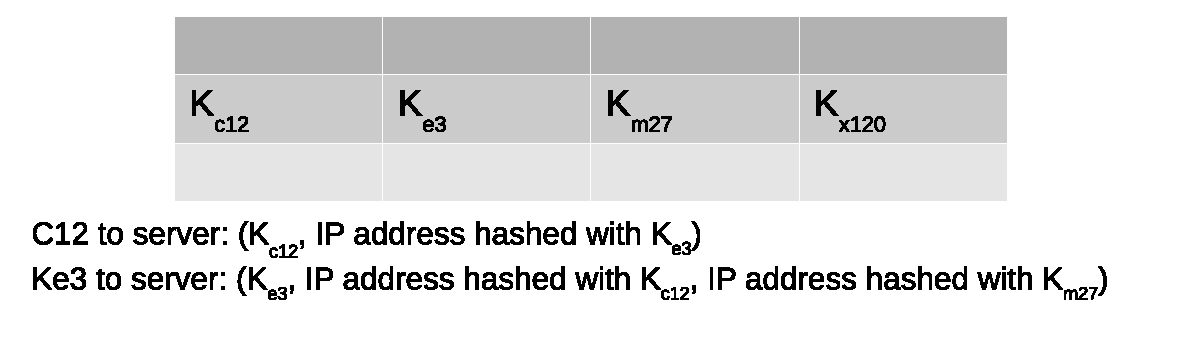
\includegraphics[scale=0.5]{address_lookup.eps}
% \caption{An Example Path Lookup}
% \end{figure}

These tuples are shuffled by the servers again. Each client and relay can then 
decrypt the IP address of their neighbours using their own public key.

The clients then have a circuit which they can use to communicate using the Tor 
protocol.

\paragraph{Circuit Signature} The Circuit Signature of the $i^{th}$ circuit in
a shuffle is the concatenation of the keys in row $i$ of the matrix: $RS_i =
M_{i0}M_{i1}M_{i2}M_{i3}$ This signature will be used in the TorCoin algorithm
to prove that TorCoins are minted only by circuits that have been assigned by
consensus groups.

\subsection{Security Considerations} 

\subsubsection{Anonymity} The TorPath protocol guarantees that no single
server can be aware of the entire circuit of any client. The anonymity set
comprises of all the clients that participate in a particular consensus group.
Groups have various sizes, allowing clients to choose the anonymity threshold
they require.

\subsubsection{Random Group Selection} The TorPath protocol increases
robustness of TorCoin to attackers. Its random group selection system prevents
attackers from deterministically placing themselves in a group. We assume that
atleast one of the assignment servers in the group is honest. In this case,
the group as a whole is able to retain privacy and anonymity. We could make
the system even more secure by randomizing group assignment, instead of just
taking temporal locality to be the only criterion.



% % Next we will descibe the consensus groups and Neff shuffle in more detail.

% % \begin{figure}[H] %   \centering %
% \includegraphics[scale=0.3]{torpath_grouping.pdf} %   \caption{TorPath Consensus
% Group Formation.} % \end{figure}

% % \subsubsection{Group Formation} % An assignment server joins a group when it
% reaches a sufficient number of clients. In practice, we expect the number to be
% modulated so that groups are being created every 10 seconds or so. To ensure
% diversity, groups must include a majority of the assignment servers on the
% network. For example, if there are ten of assignment servers on the entire
% network, a consensus group requires at least six.

% % Once a consensus group exists, it splits into three decentralized shuffle
% % sets, each responsible for assigning a different relay to clients. An
% % $n$-client shuffle set has $n$ rows, each pointing to a possible relay. For
% % example, shuffle sets $s_0$, $s_1$, and $s_2$ could be responsible for
% % assigning entry, middle, and exit relays to clients.

% % \subsubsection{Neff Shuffles for Circuit Assignment} % Each shuffle set runs a
% Neff shuffle ~\cite{neff2001verifiable} to shuffle its list of $n$ relays, so
% that it can assign each relay $i$ to client $i$. Each client receives a tuple
% $(r_0, r_1, r_2, s)$ specifying the address of entry, middle, and exit relays,
% along with a circuit signature.

% % \begin{figure} %   \centering %
% \includegraphics[scale=0.3]{torpath_shufflesets.pdf} %   \caption{Each Shuffle
% Set carries out its own Neff shuffle to determine one part of the path.} %
% \end{figure}

% % \subsubsection{TorCoin Verification} % Assignment servers input circuit
% signatures into a cryptographic accumulator, and publish that list of
% accumulators. Anyone can verify that a circuit existed at least once, simply by
% searching for a signature.

% % \subsubsection{Decoupled Protocol} % The TorPath protocol only replaces
% directory servers. Therefore, implementing it does not require modifying any Tor
% code. So clients can use the TorPath protocol for circuit assignment then
% communicate using the existing Tor protocol.
